\smallframetitle

\section{From 22/07/24 to 26/07/24}
\insertsectionframe

\subsection{Further advancement on road detection}
\insertsubsectionframe

\begin{frame}{Adjustements in the method}
    \begin{block}{Stop using the angle criterion}
        After analysing last week's results, I decided to stop using the angle criterion because it doesn't delete the right edges.
        Therefore, I fine-tuned the weight calculation method, so that it doesn't need it anymore
    \end{block}
    \begin{block}{New edge weight calculation}
        For each couple of cities, we compute a weight using this formula :
        $$w_{\text{city1, city2}} = \frac{(\min(\text{size(city1)},\text{size(city2)}))^{1.3}}{(\text{dist(city1, city2)})^{1.2}}$$
        With the size of a city refering to the number of base stations detected inside that city.
    \end{block}
\end{frame}

\begin{frame}{Results}
    \begin{columns}
        \begin{column}{0.5\textwidth}
            \begin{figure}
                \includegraphics[height=0.3\paperwidth]{images/road\_detection/edges\_weight\_filtration\_refined.png}
                \caption{weight filtration with new calculation, cap value = $0.2$}
            \end{figure}
        \end{column}
        \begin{column}{0.5\textwidth}
            \begin{figure}
                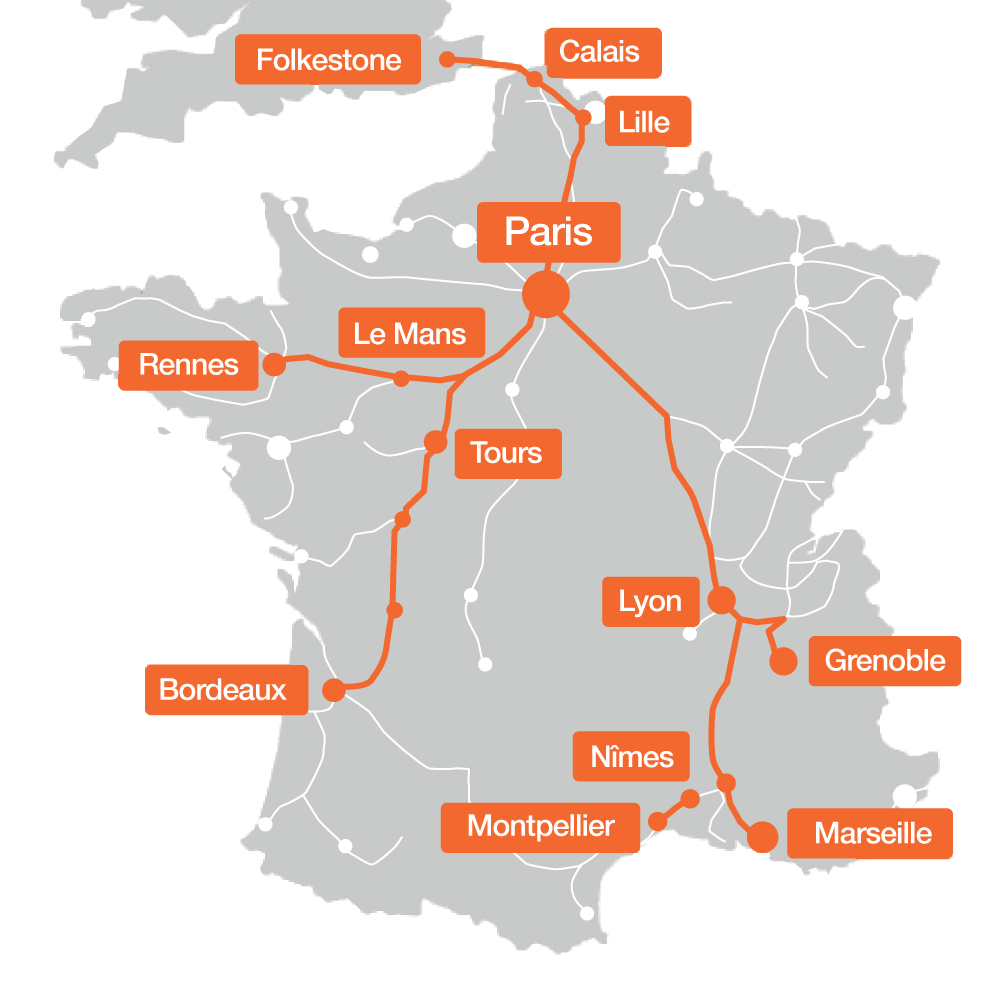
\includegraphics[height=0.3\paperwidth]{images/road\_detection/tgv-4g.png}
                \caption{TGV lines covered in 4G by Orange}
            \end{figure}
        \end{column}
    \end{columns}        
\end{frame}

\subsection{State of the art of our different neighbouring methods}
\insertsubsectionframe

\begin{frame}{Delaunay and simple criteria}
    \begin{block}{Principle of the method}
        At first we will apply a Delaunay triangulation, to have a potential neighbours graph, and, afterwards, we apply the simple criteria : distance, angle and quadrant,
        to filter the bad neighbouring connexions.
    \end{block}

    \begin{block}{Criteria}
        \begin{itemize}
            \item Distance: we filter every edge longer than $\unit[15]{km}$;
            \item Angle : we filter every edge separated from the nearest one by an angle more narrow than $20^\circ$;
            \item Quadrant : we filter according to the simple quadrant criterion.
        \end{itemize}
    \end{block}
\end{frame}

\begin{frame}{Delaunay and simple criteria - pros and cons}
    \begin{block}{Pros}
        \begin{itemize}
            \item Every edge is treated equally, wether it in countryside or in a city;
            \item This method is really simple to put in place.
        \end{itemize}
    \end{block}

    \begin{block}{Cons}
        \begin{itemize}
            \item Every edge is treated equally, wether it in countryside or in a city. This leads to non precise results.
        \end{itemize}
    \end{block}
\end{frame}

\begin{frame}{Delaunay and enhanced criteria}
    \begin{block}{Principle of the method}
        At first we will apply a Delaunay triangulation, to have a potential neighbours graph, and, afterwards, we apply the enhanced criteria : distance, angle and quadrant,
        to filter the bad neighbouring connexions. Same principle as before but we will take in account if a city is in or not in a city.
    \end{block}

    \begin{block}{3NN cityness classification method}
        To classify each base station we need a method. Here, we will take the mean distance to the 3 nearest neighbours.

        Let's call this value $\gamma$, in $\unit{km}$. So, we have 4 different categories.
        For each category, we will apply a different distance and angle criterion :
        \begin{itemize}
            \item $\gamma\in\left]0, 1\right]$ : city center ($\text{max\_distance}=\unit[2]{km}$, $\text{min\_angle}=5^\circ$);
            \item $\gamma\in\left]1, 2\right]$ : urban area ($\text{max\_distance}=\unit[5]{km}$, $\text{min\_angle}=15^\circ$);
            \item $\gamma\in\left]2, 4\right]$ : extra-urban area ($\text{max\_distance}=\unit[10]{km}$, $\text{min\_angle}=25^\circ$);
            \item $\gamma\in\left]4, \infty\right[$ : courntryside ($\text{max\_distance}=\unit[15]{km}$, $\text{min\_angle}=30^\circ$).
        \end{itemize}
    \end{block}

    And then, of course, we apply the enhanced quadrant criterion.
\end{frame}

\begin{frame}{Delaunay and enhanced criteria - pros and cons}
    \begin{block}{Pros}
        \begin{itemize}
            \item We take in account the \og cityness\fg{} of each base station to compute its neighbours.
        \end{itemize}
    \end{block}

    \begin{block}{Cons}
        \begin{itemize}
            \item We have no method to be sure that we choose the correct distances and angles;
            \item The filtering does not seems good sometimes. On one hand we filter too much and on the other hand, we filter too less.
        \end{itemize}
    \end{block}

    Those problems could come from the Delaunay triangulation, which is maybe not the base for this use case.
\end{frame}

\begin{frame}{Gabriel graph and enhanced criteria}
    \begin{block}{Principle of the method}
        At first we will create a potential neighbours graph : the Gabriel graph and, afterwards, we apply the enhanced criteria : distance, angle and quadrant,
        to filter the bad neighbouring connexions. Same principle as before but we apply a pre-filtering with the Gabriel graph.
    \end{block}

    \begin{block}{Gabriel graph\footnotemark}
        A Gabriel graph is a subgraph of a Delaunay triangulation. Formally, it is the graph $G$ with vertex set $S$
        in which any two distinct points $p\in S$ and $q\in S$ are adjacent precisely when the closed disc having $pq$ as a diameter contains no other points.
    \end{block}

    And then, of course, we apply the enhanced criteria, as listed before.

    \footnotetext{\url{https://en.wikipedia.org/wiki/Gabriel\_graph}}
\end{frame}

\begin{frame}{Gabriel graph and enhanced criteria - pros and cons}
    \begin{block}{Pros}
        \begin{itemize}
            \item We add another level of filtering.
        \end{itemize}
    \end{block}

    \begin{block}{Cons}
        \begin{itemize}
            \item We add another level of complexity.
        \end{itemize}
    \end{block}

    This is not perfect, maybe we can get rid of the Delaunay triangulation.
\end{frame}

\begin{frame}{$k$-NN and enhanced criteria}
    \begin{block}{Principle of the method}
        At first we will create a potential neighbours graph with the $k$-NN method and, afterwards, we apply the enhanced criteria : distance, angle and quadrant,
        to filter the bad neighbouring connexions.
    \end{block}

    \begin{block}{$k$-NN\footnotemark}
        To create this graph we will, for each base station, connect it to its $k$ nearest neighbours.
    \end{block}

    And then, of course, we apply the enhanced criteria, as listed before.

    \footnotetext{\url{https://scikit-learn.org/stable/modules/generated/sklearn.neighbors.NearestNeighbors.html}}
\end{frame}

\begin{frame}{Gabriel graph and enhanced criteria - pros and cons}
    \begin{block}{Pros}
        \begin{itemize}
            \item We get rid of the Delaunay traingulation, so we could connect more base stations.
        \end{itemize}
    \end{block}

    \begin{block}{Cons}
        \begin{itemize}
            \item A lot of edges to filter;
            \item The filtering methods is maybe not adapted.
        \end{itemize}
    \end{block}

    This is not perfect, but got rid of the Delaunay triangulation.
\end{frame}